\documentclass{article}
\usepackage[utf8]{inputenc}
\usepackage[norsk]{babel}
\usepackage{mathtools} 
\usepackage{hyperref}
\usepackage{listings} 
\usepackage{graphicx}
\begin{document}
\begin{titlepage}
\begin{center}

\vspace*{3cm}
\textsc{\Huge D2b}\\[0.7cm]
\textsc{\medium TTM4100 - Communication Services and Networks}\\[0.3cm]
\textsc{\medium TDT4140 - Software Enigneering}\\[0.3cm]
\textsc{\medium TDT4145 - Data Modeling, Databases and Database Management Systems}\\[0.3cm]
\textsc{\medium TDT4180 - Human-Computer Interaction}\\[0.3cm]

\textbf{\Large Gruppe 7:} \\[0.2cm]
\text{\Large Espen Albert, Finn Inderhaug, Kristoffer Andreas Dalby} \\
\text{\Large Christoffer B. Nysæter, Andreas Wien, Jonas André Dalseth}\\[1cm]

\today

\end{center}
\end{titlepage}



\section{Description of the prototype}
% remember to put graphs har, use \begin{figure } from wiki
\begin{figure}[h!] 
    \begin{center} 
        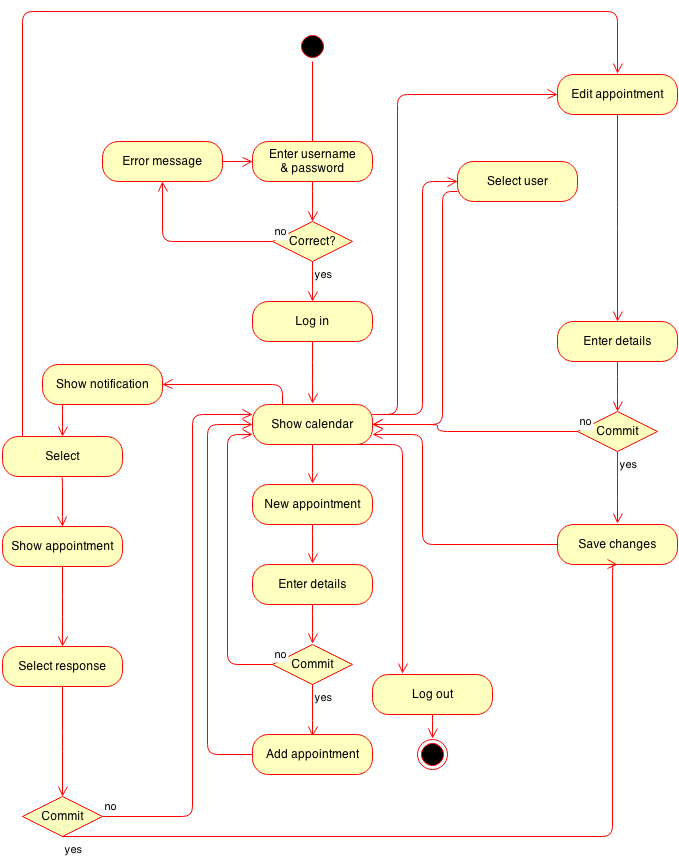
\includegraphics[width=8cm]{img/calendarStateDiagram.png}
        \caption{Calendar state diagram}
    \label{calendarstatediagram}
    \end{center}
\end{figure}

\newpage

\begin{figure}[h!] 
    \begin{center} 
        \includegraphics[width=8cm]{img/IMG_5600.png}
        \caption{Log in screen}
    \label{login}
    \end{center}
\end{figure}
This is the loginscreen. From here the user can enter the username and password. To log in, the user can press the ``Log in''-button.

\begin{figure}[h!] 
    \begin{center} 
        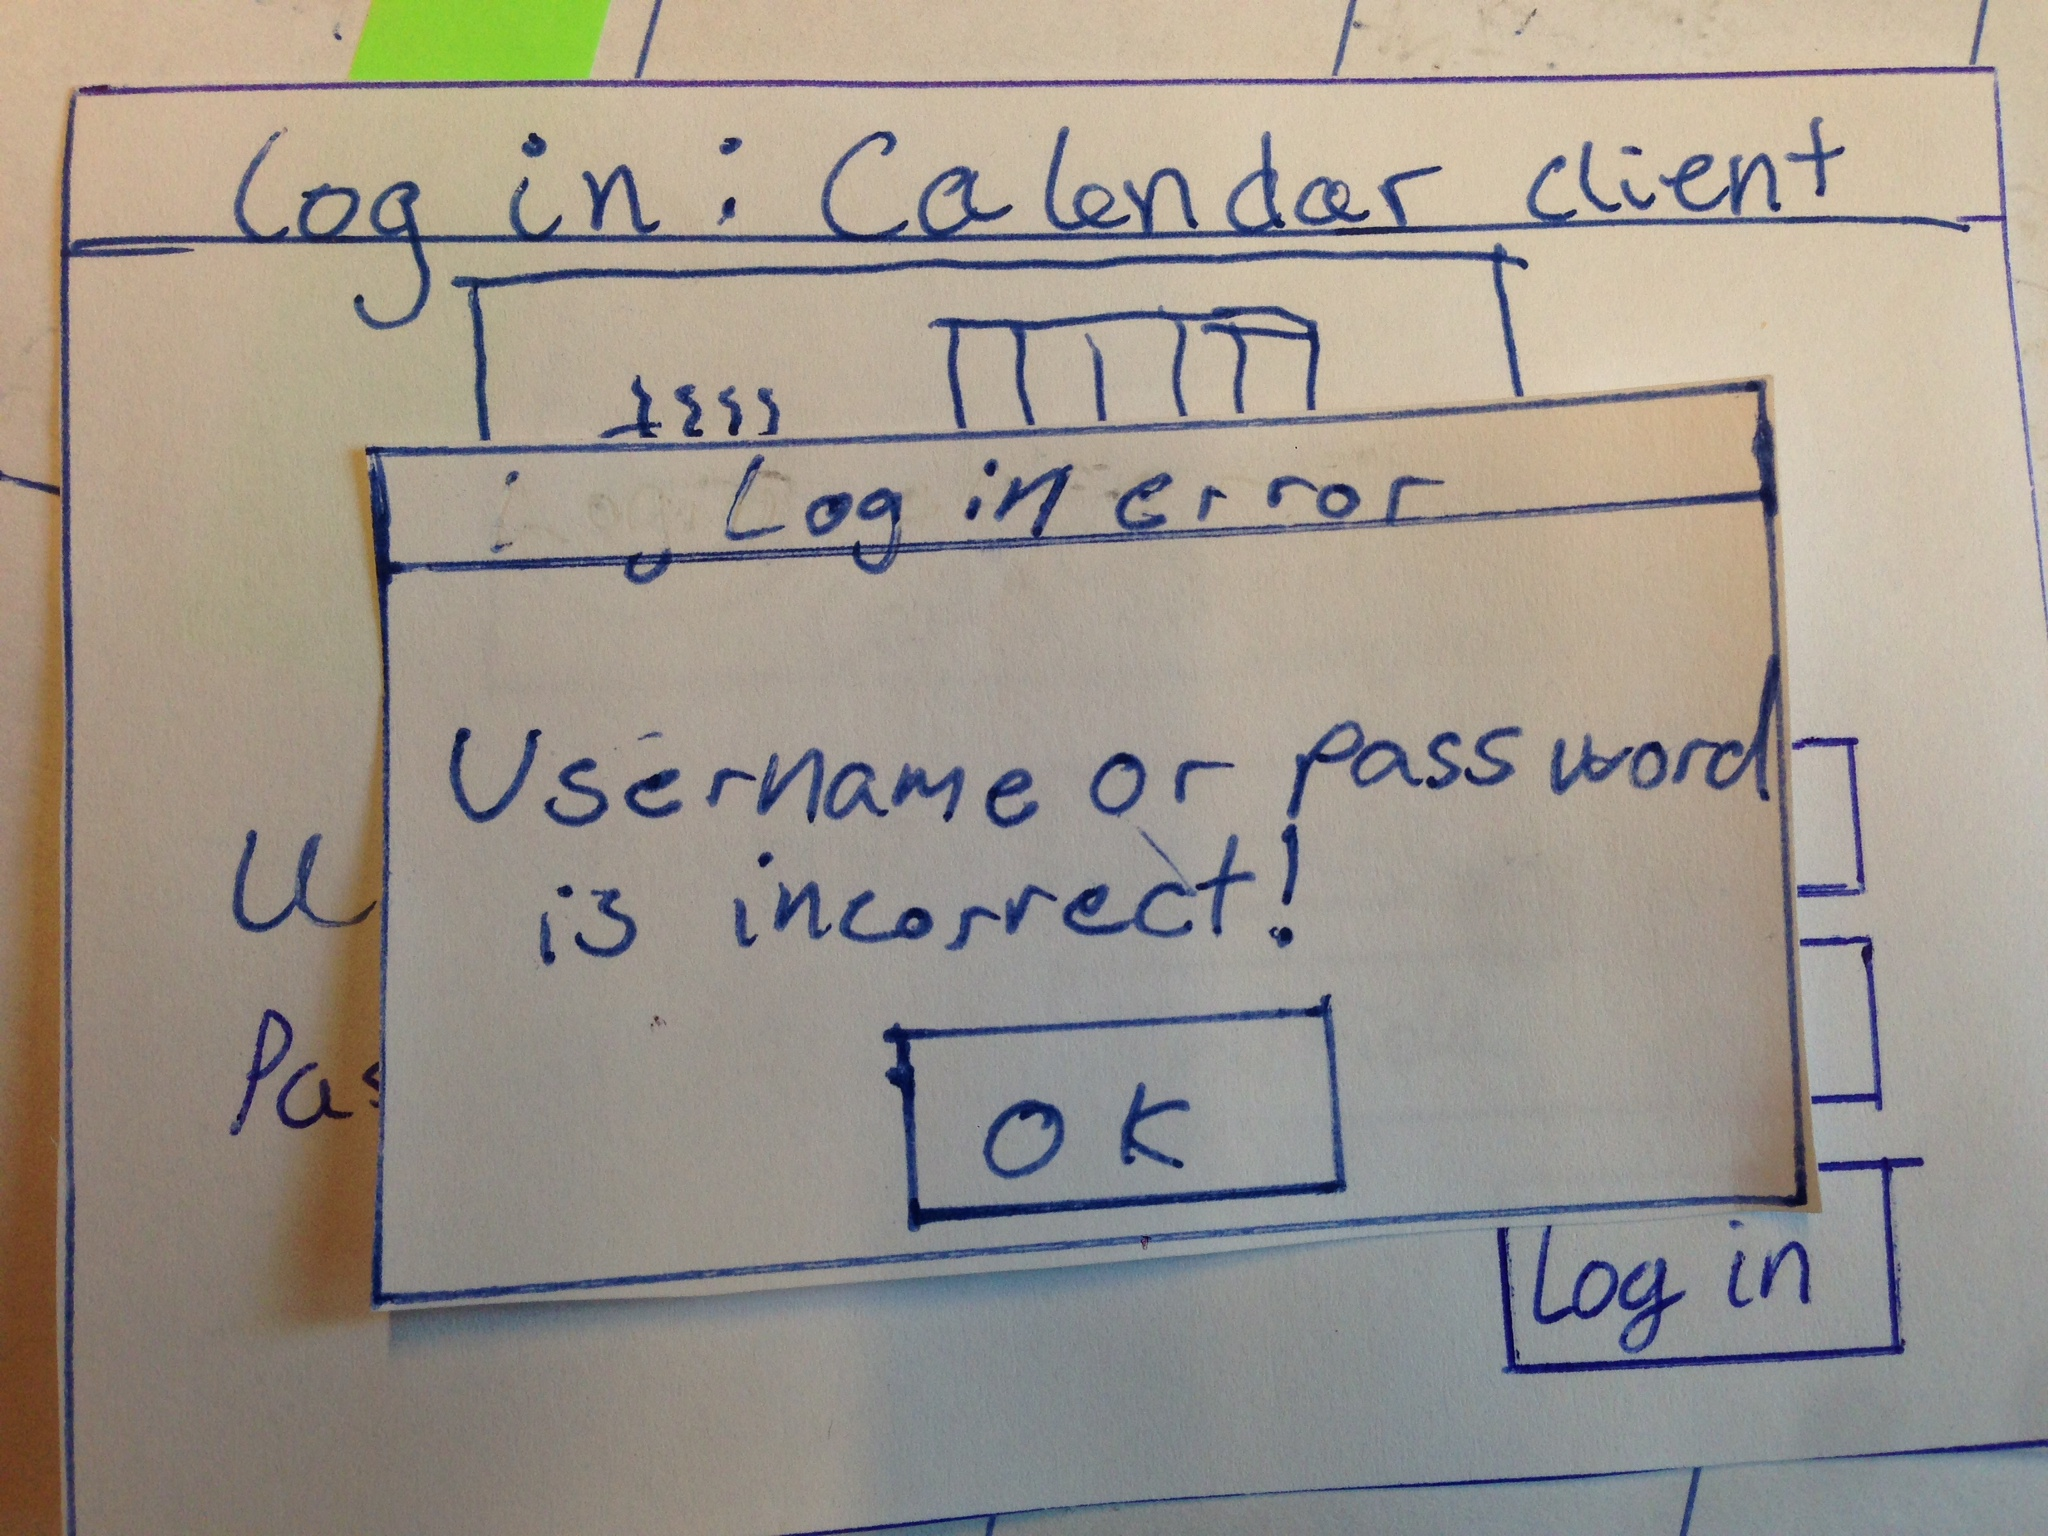
\includegraphics[width=8cm]{img/IMG_5612.JPG}
        \caption{Log in error}
    \label{loginerror}
    \end{center}
\end{figure}
If the username and/or password i incorrect, this popup screen will appear. When the ``OK''-button is pressed, the error will close.

\newpage

\begin{figure}[h!] 
    \begin{center} 
        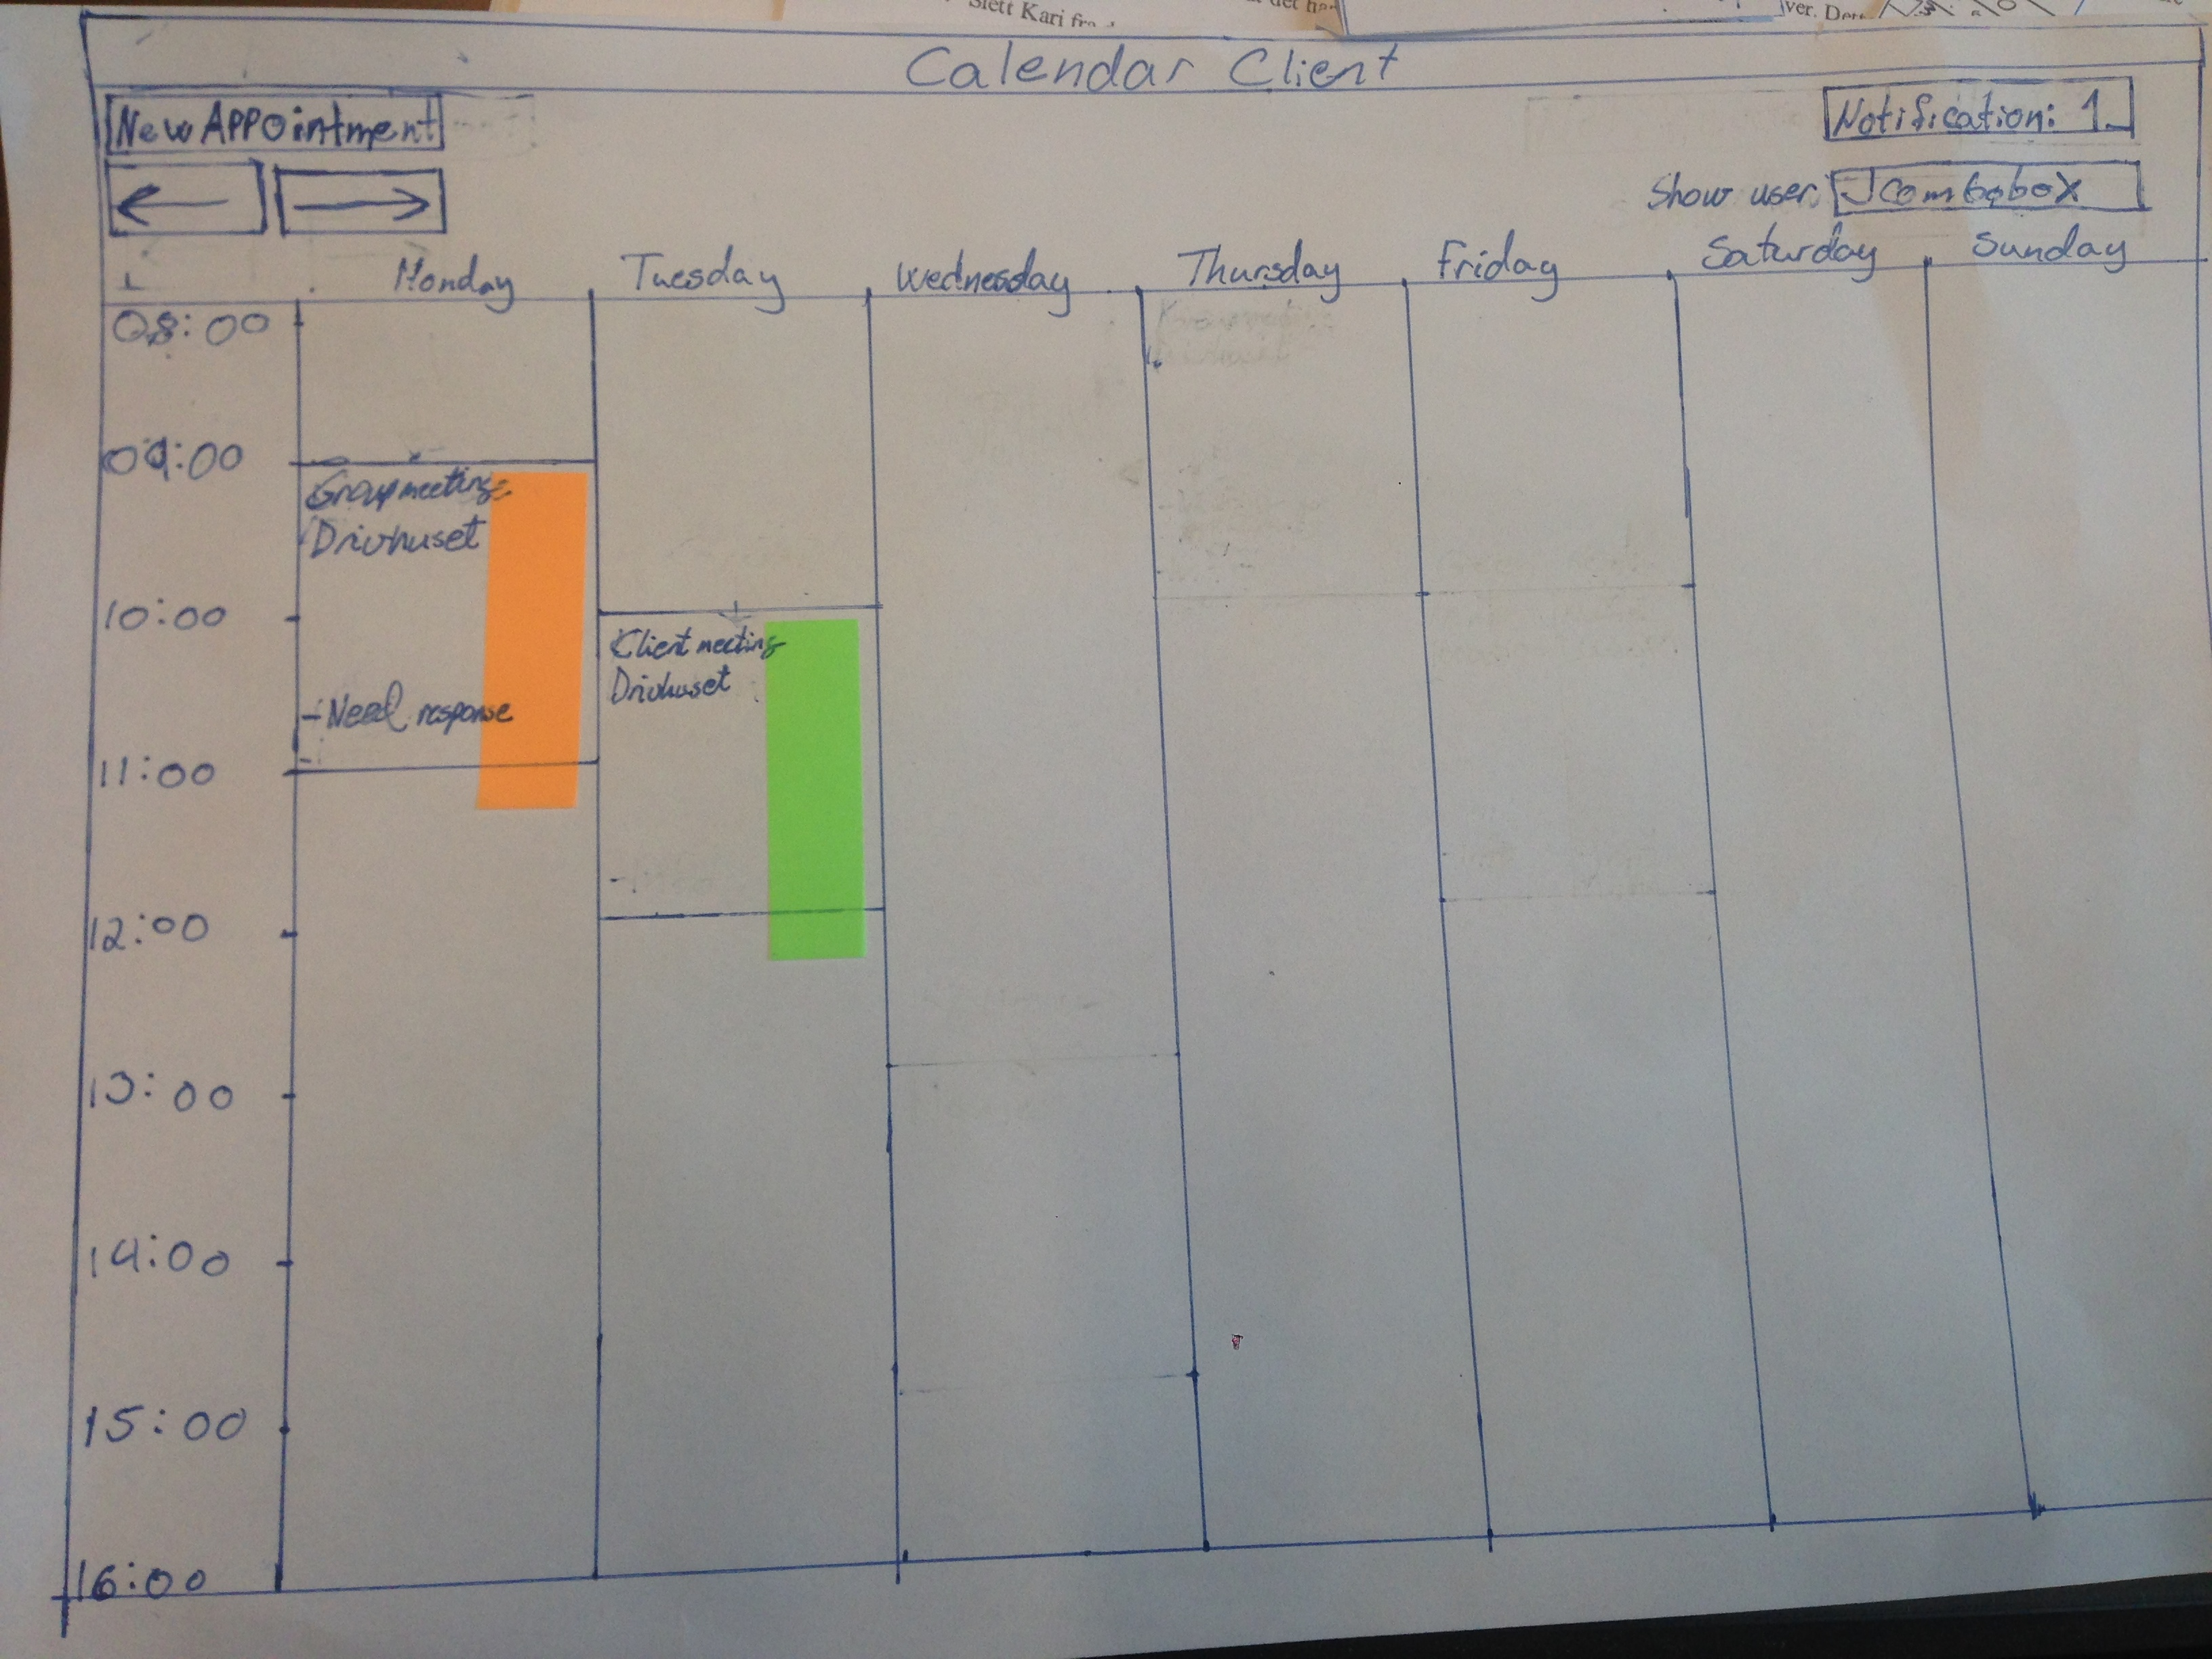
\includegraphics[width=8cm]{img/IMG_5601.JPG}
        \caption{Week view}
    \label{weekview}
    \end{center}
\end{figure}

This is the main screen. In this screen, the user can view his/her appoinments. By pressing the ``new  appointment'' - button, the user can make a new appointment. When pressing the arrow-buttons, the user can see the previous or next week. By pressing an appointment, the user can edit or view an appointment. The ``notification''-button make it possible to view the users notification.

\begin{figure}[h!] 
    \begin{center} 
        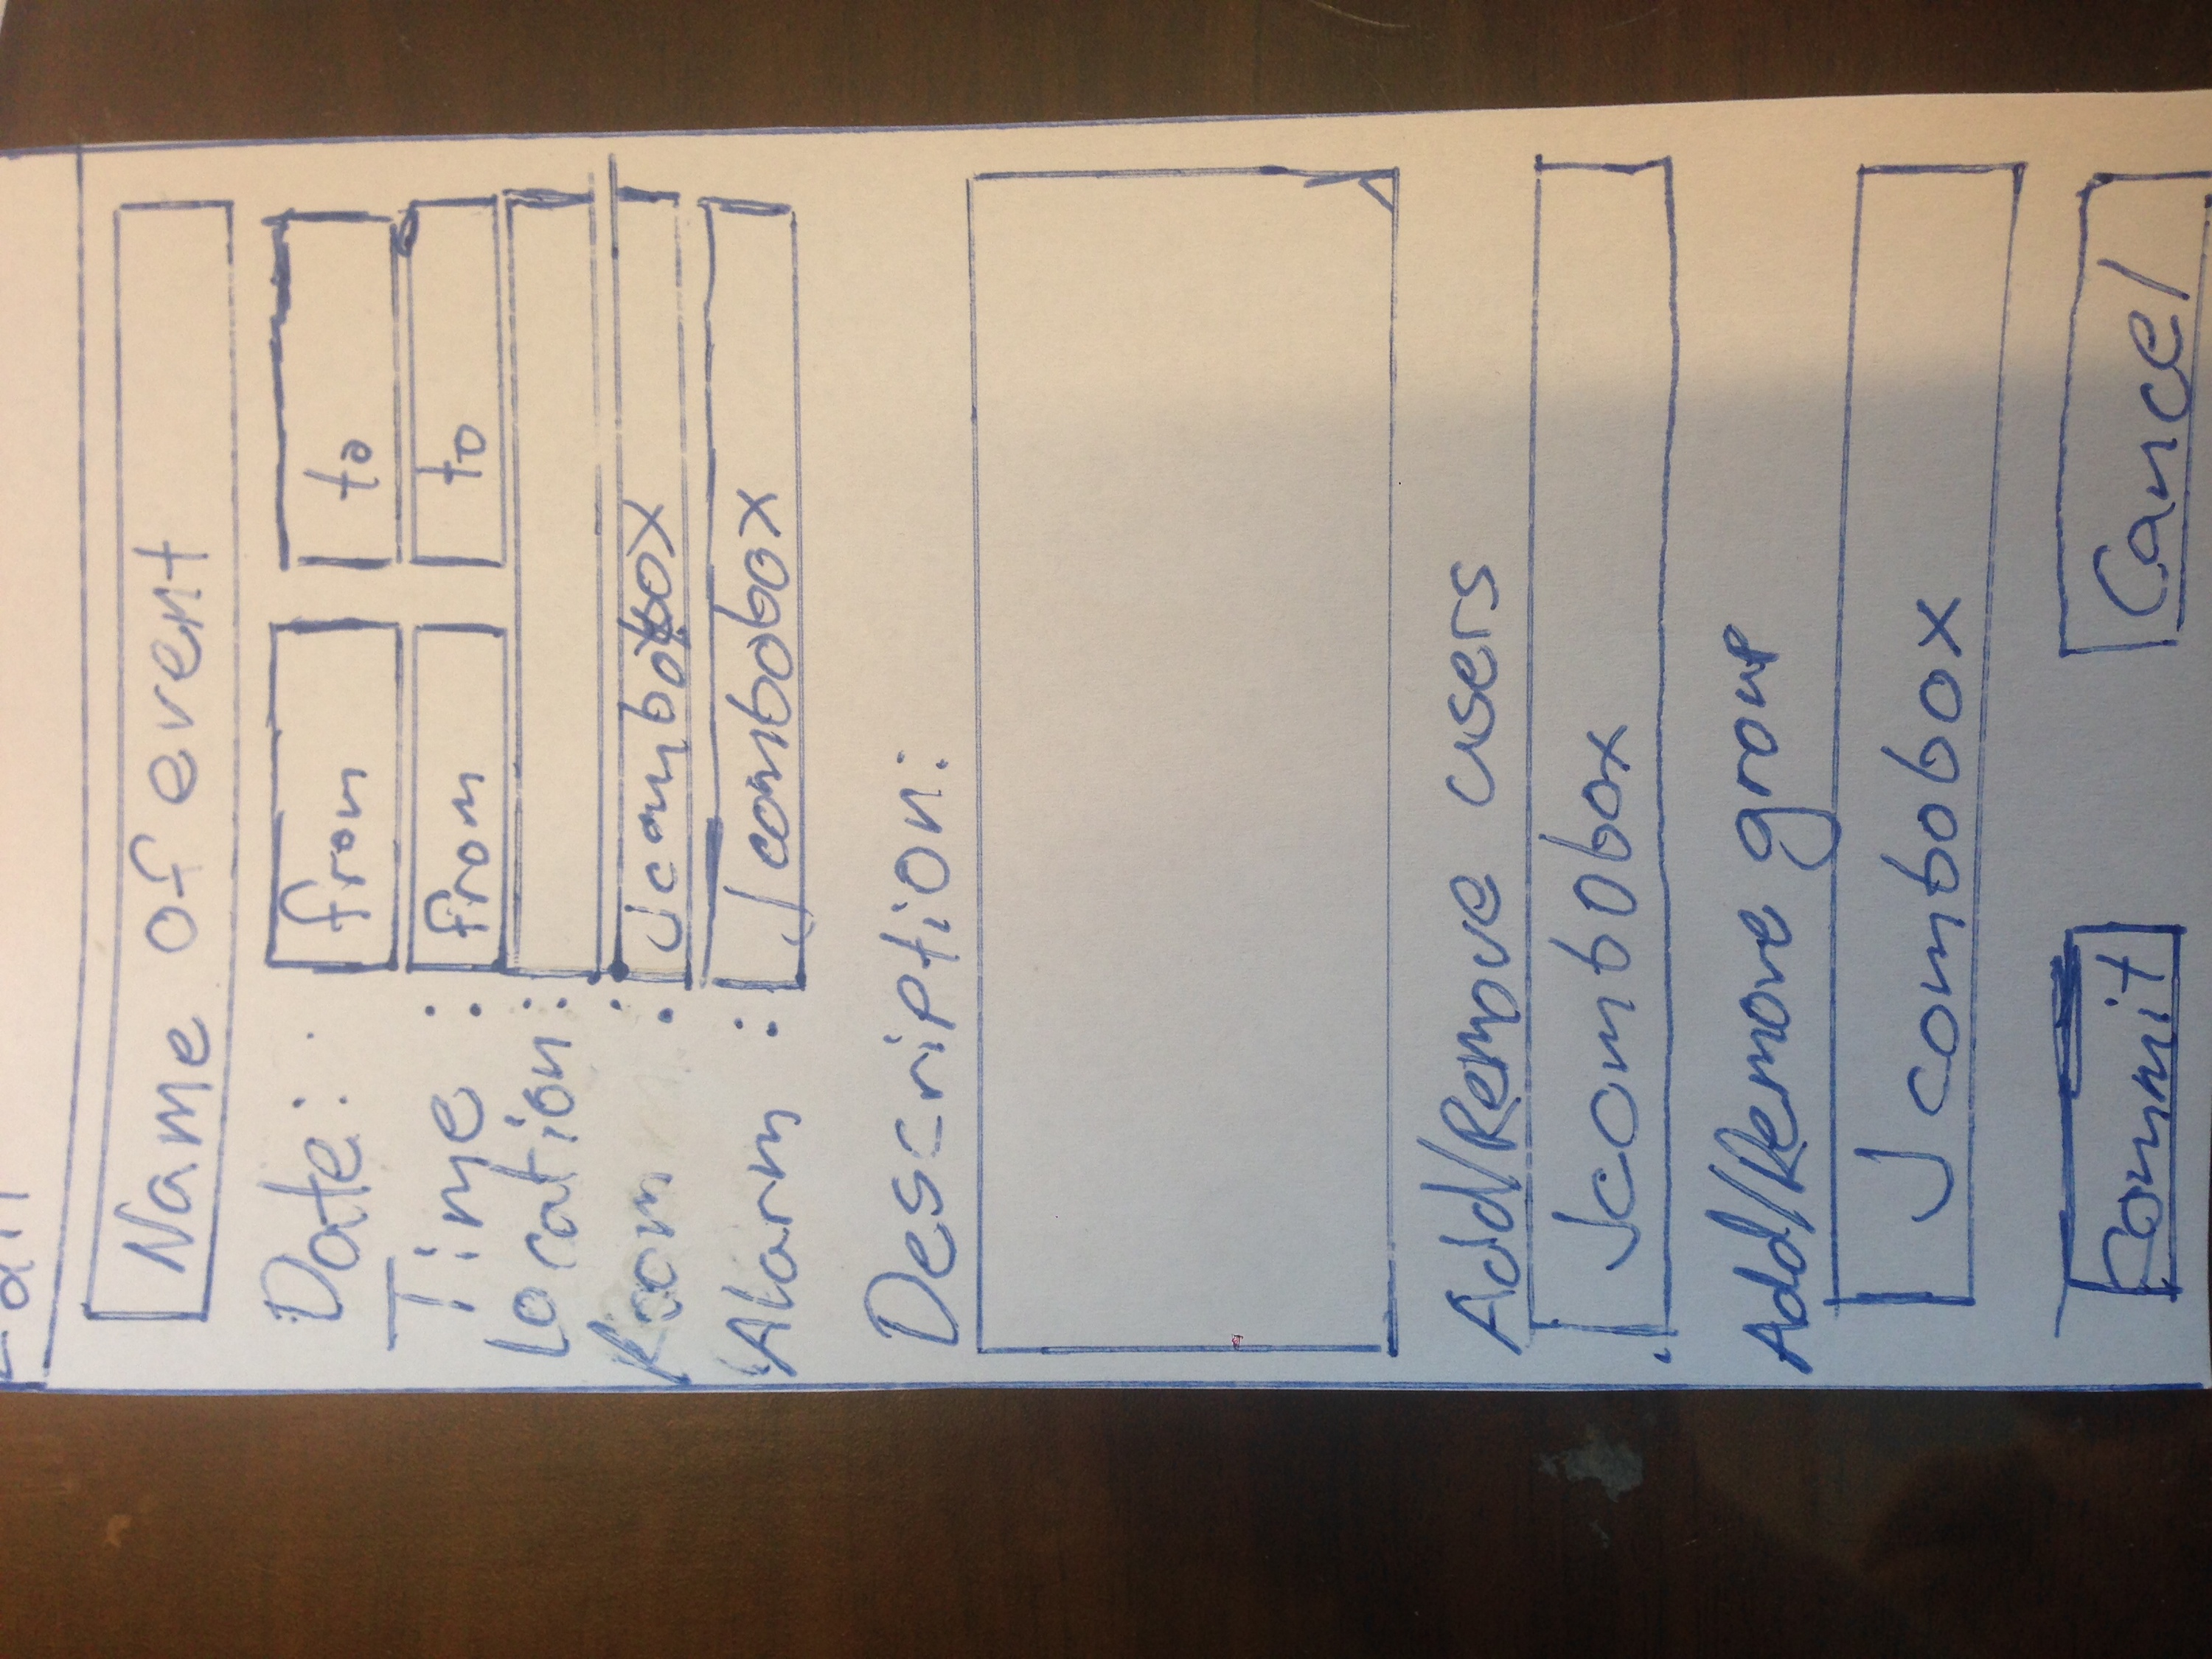
\includegraphics[width=8cm]{img/IMG_5602.JPG}
        \caption{Edit screen}
    \label{edit}
    \end{center}
\end{figure}
In the edit-screen, the user can make new appointments/change the existing ones. Date, time, room and alarm can be set from a dropdown menu, while location and description is textfields where the user can enter text. By pressing the ``commit''-button, the appointment will be made.

\newpage

\begin{figure}[h!] 
    \begin{center} 
        \includegraphics[width=8cm]{img/IMG_5604.png}
        \caption{Room dropdown menu}
    \label{roomdropdown}
    \end{center}
\end{figure}
This is an example of a dropdown menu. In this one, the user reserves a room.

\newpage

\begin{figure}[h!] 
    \begin{center} 
        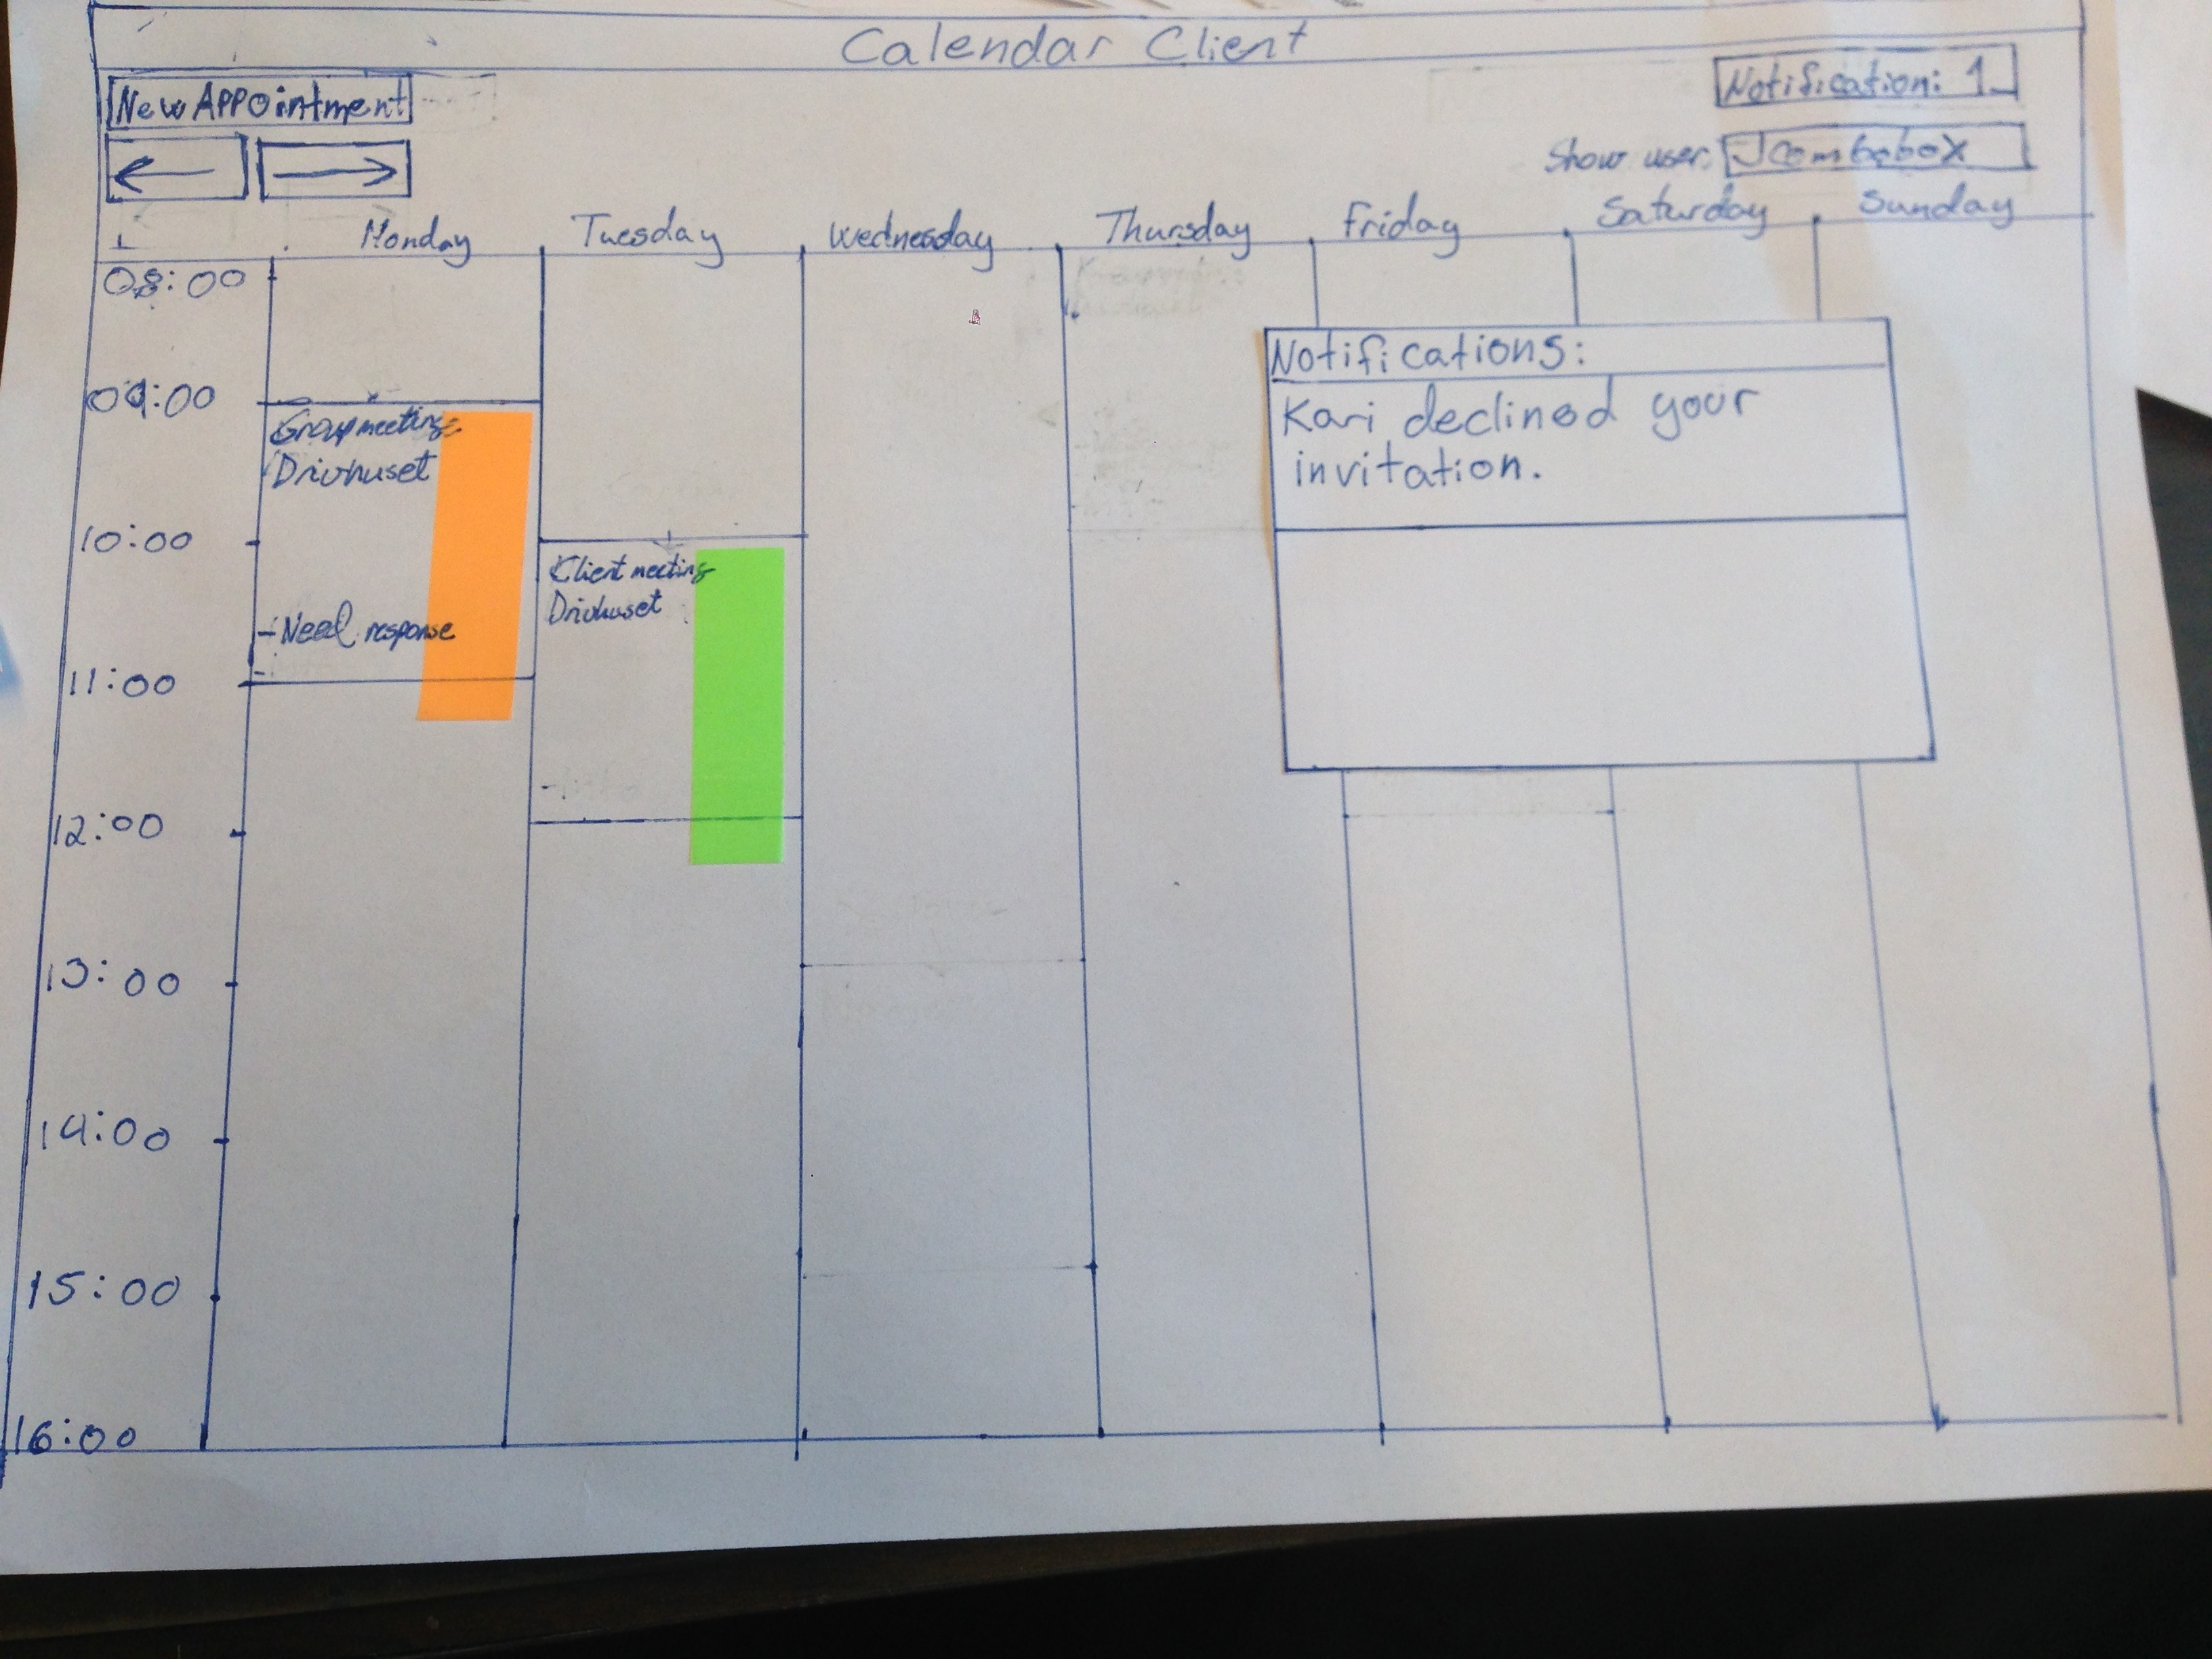
\includegraphics[width=8cm]{img/IMG_5608.JPG}
        \caption{Notification screen}
    \label{notificationscreen}
    \end{center}
\end{figure}
In the notification-window, the users appoiments are view. If the different appointmets are clicked, the user will be sendt directly to the appointment connected to the notification.

\newpage

\begin{figure}[h!] 
    \begin{center} 
        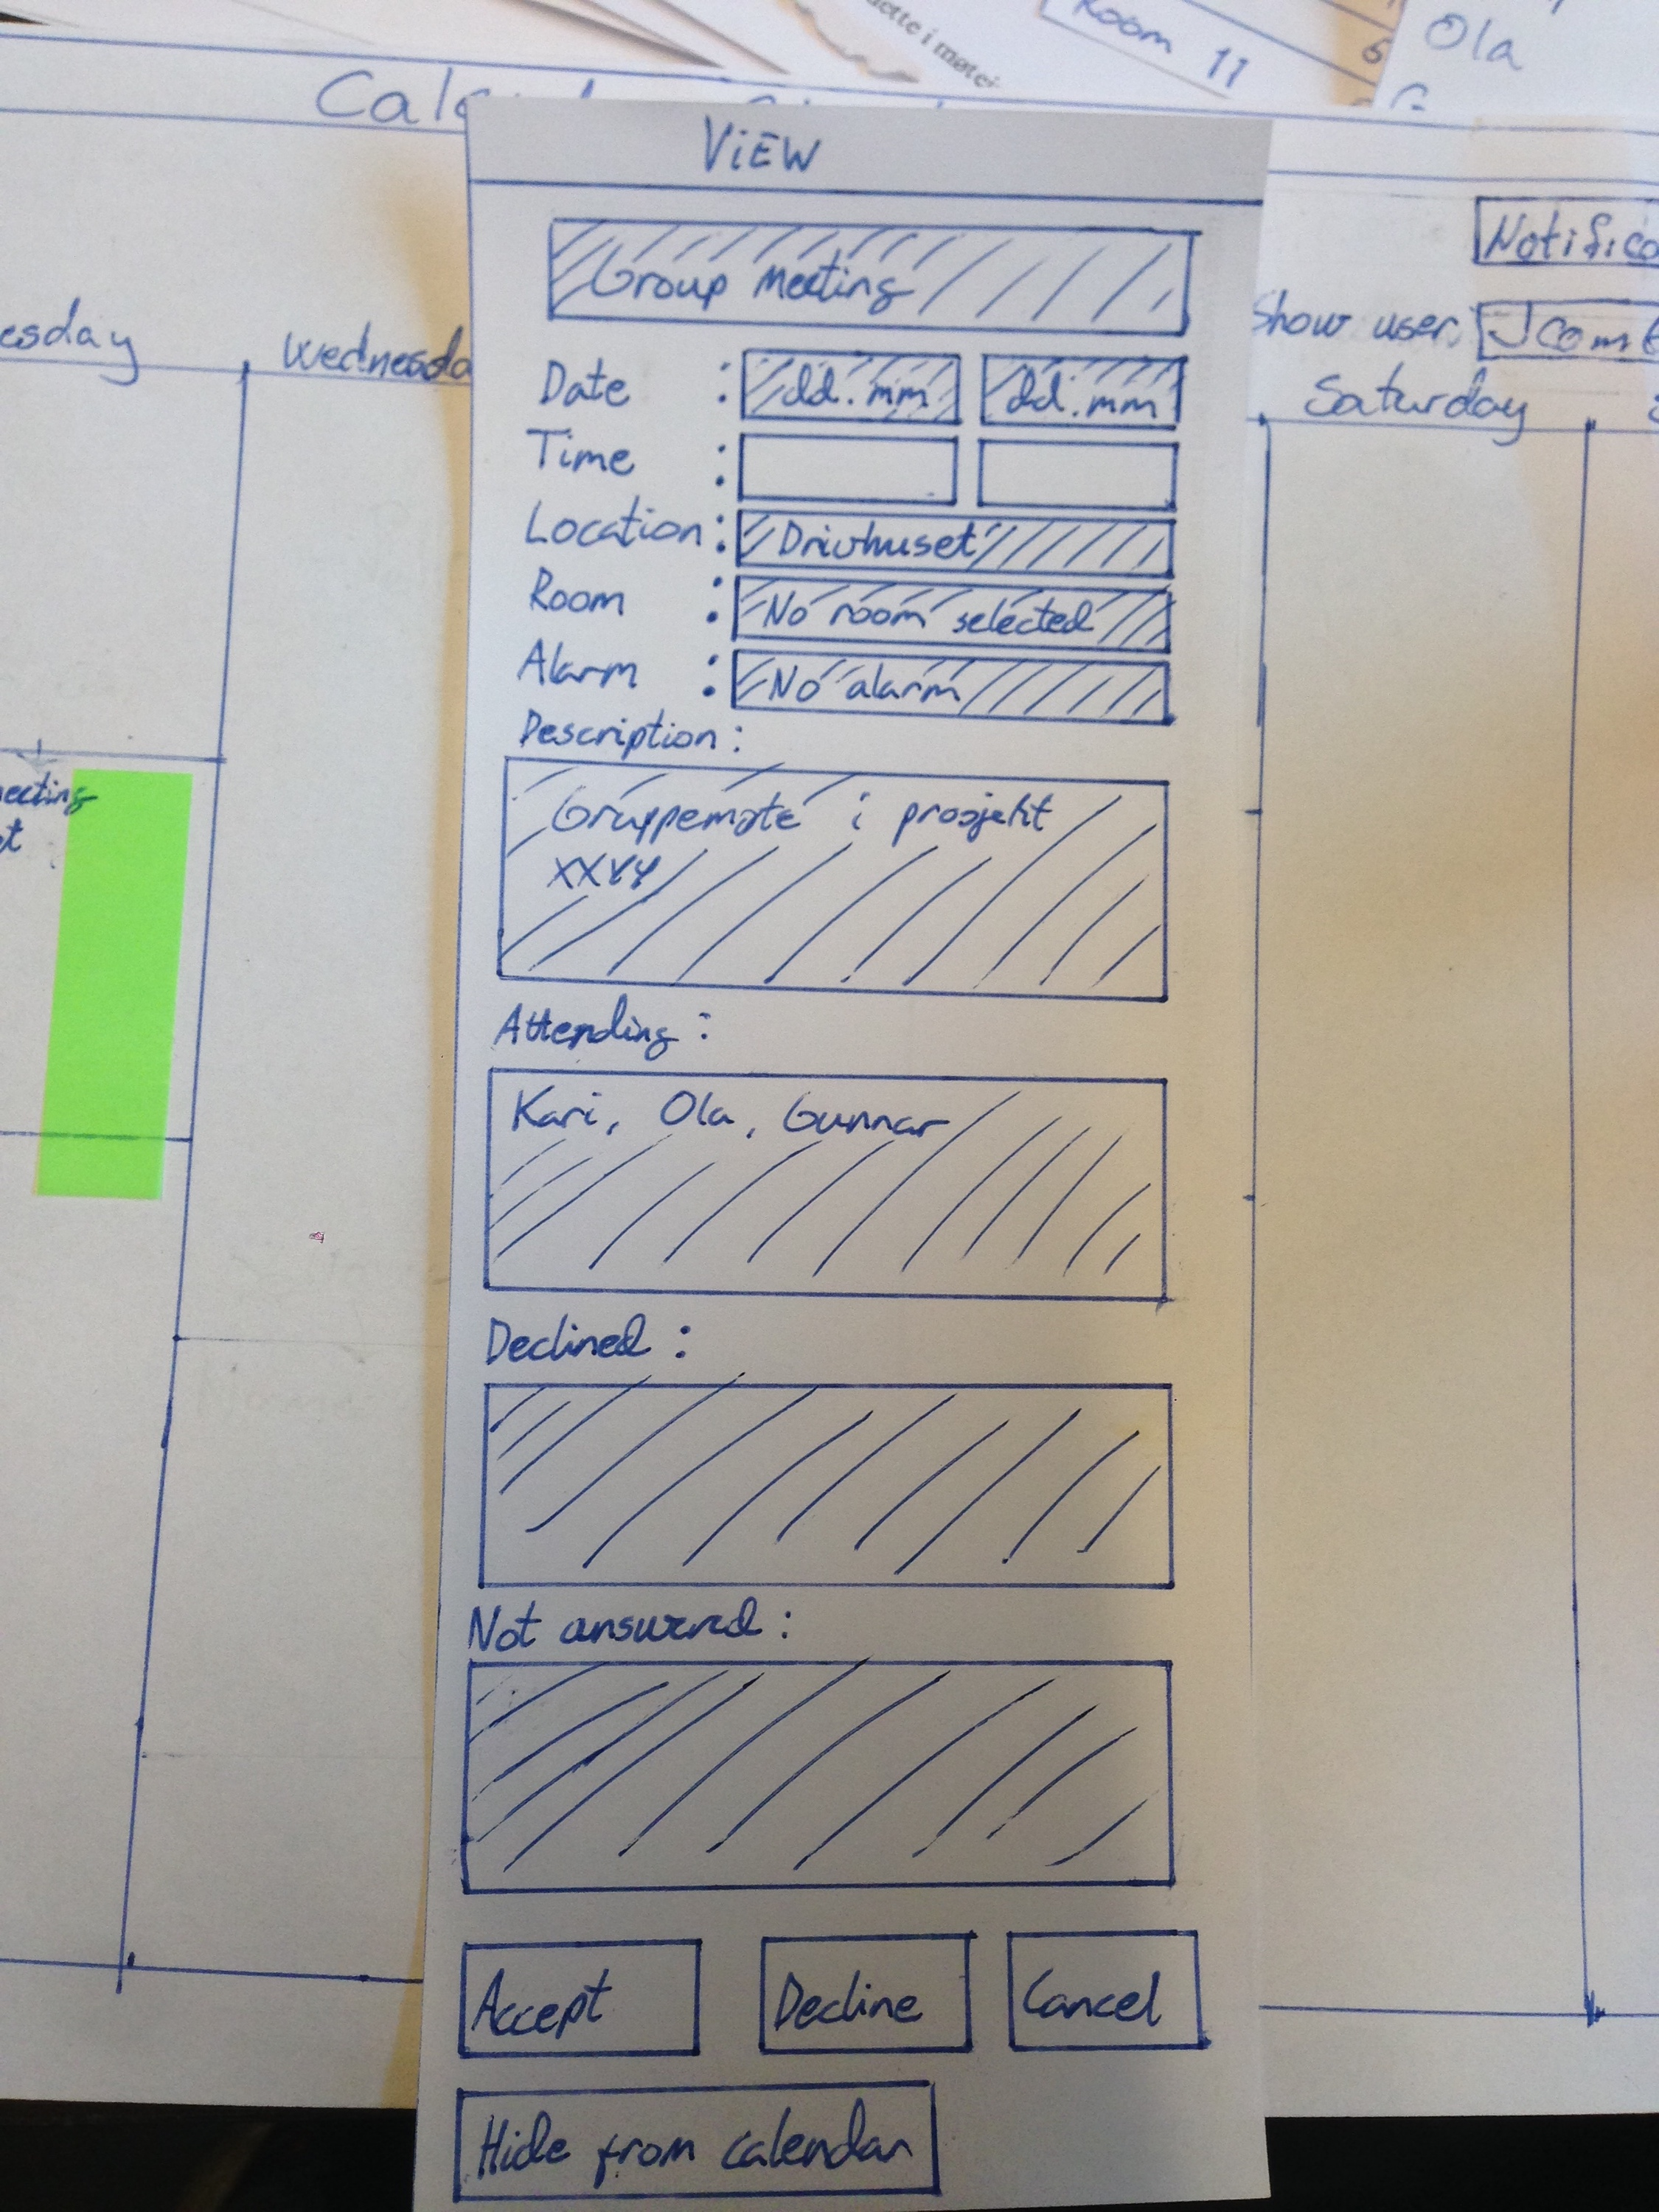
\includegraphics[width=8cm]{img/IMG_5609.JPG}
        \caption{View screen}
    \label{view}
    \end{center}
\end{figure}
In this screen the user can view an appointment, in addition make a response if she will attend or not, by using the ``Accept''-button og ``Decline''-button. By pressing cancel the window will close, and no changes will be made. If the user press the ``Hide from calendar''-button, the appointment will be hided from the users calendar.

\newpage

\begin{figure}[h!] 
    \begin{center} 
        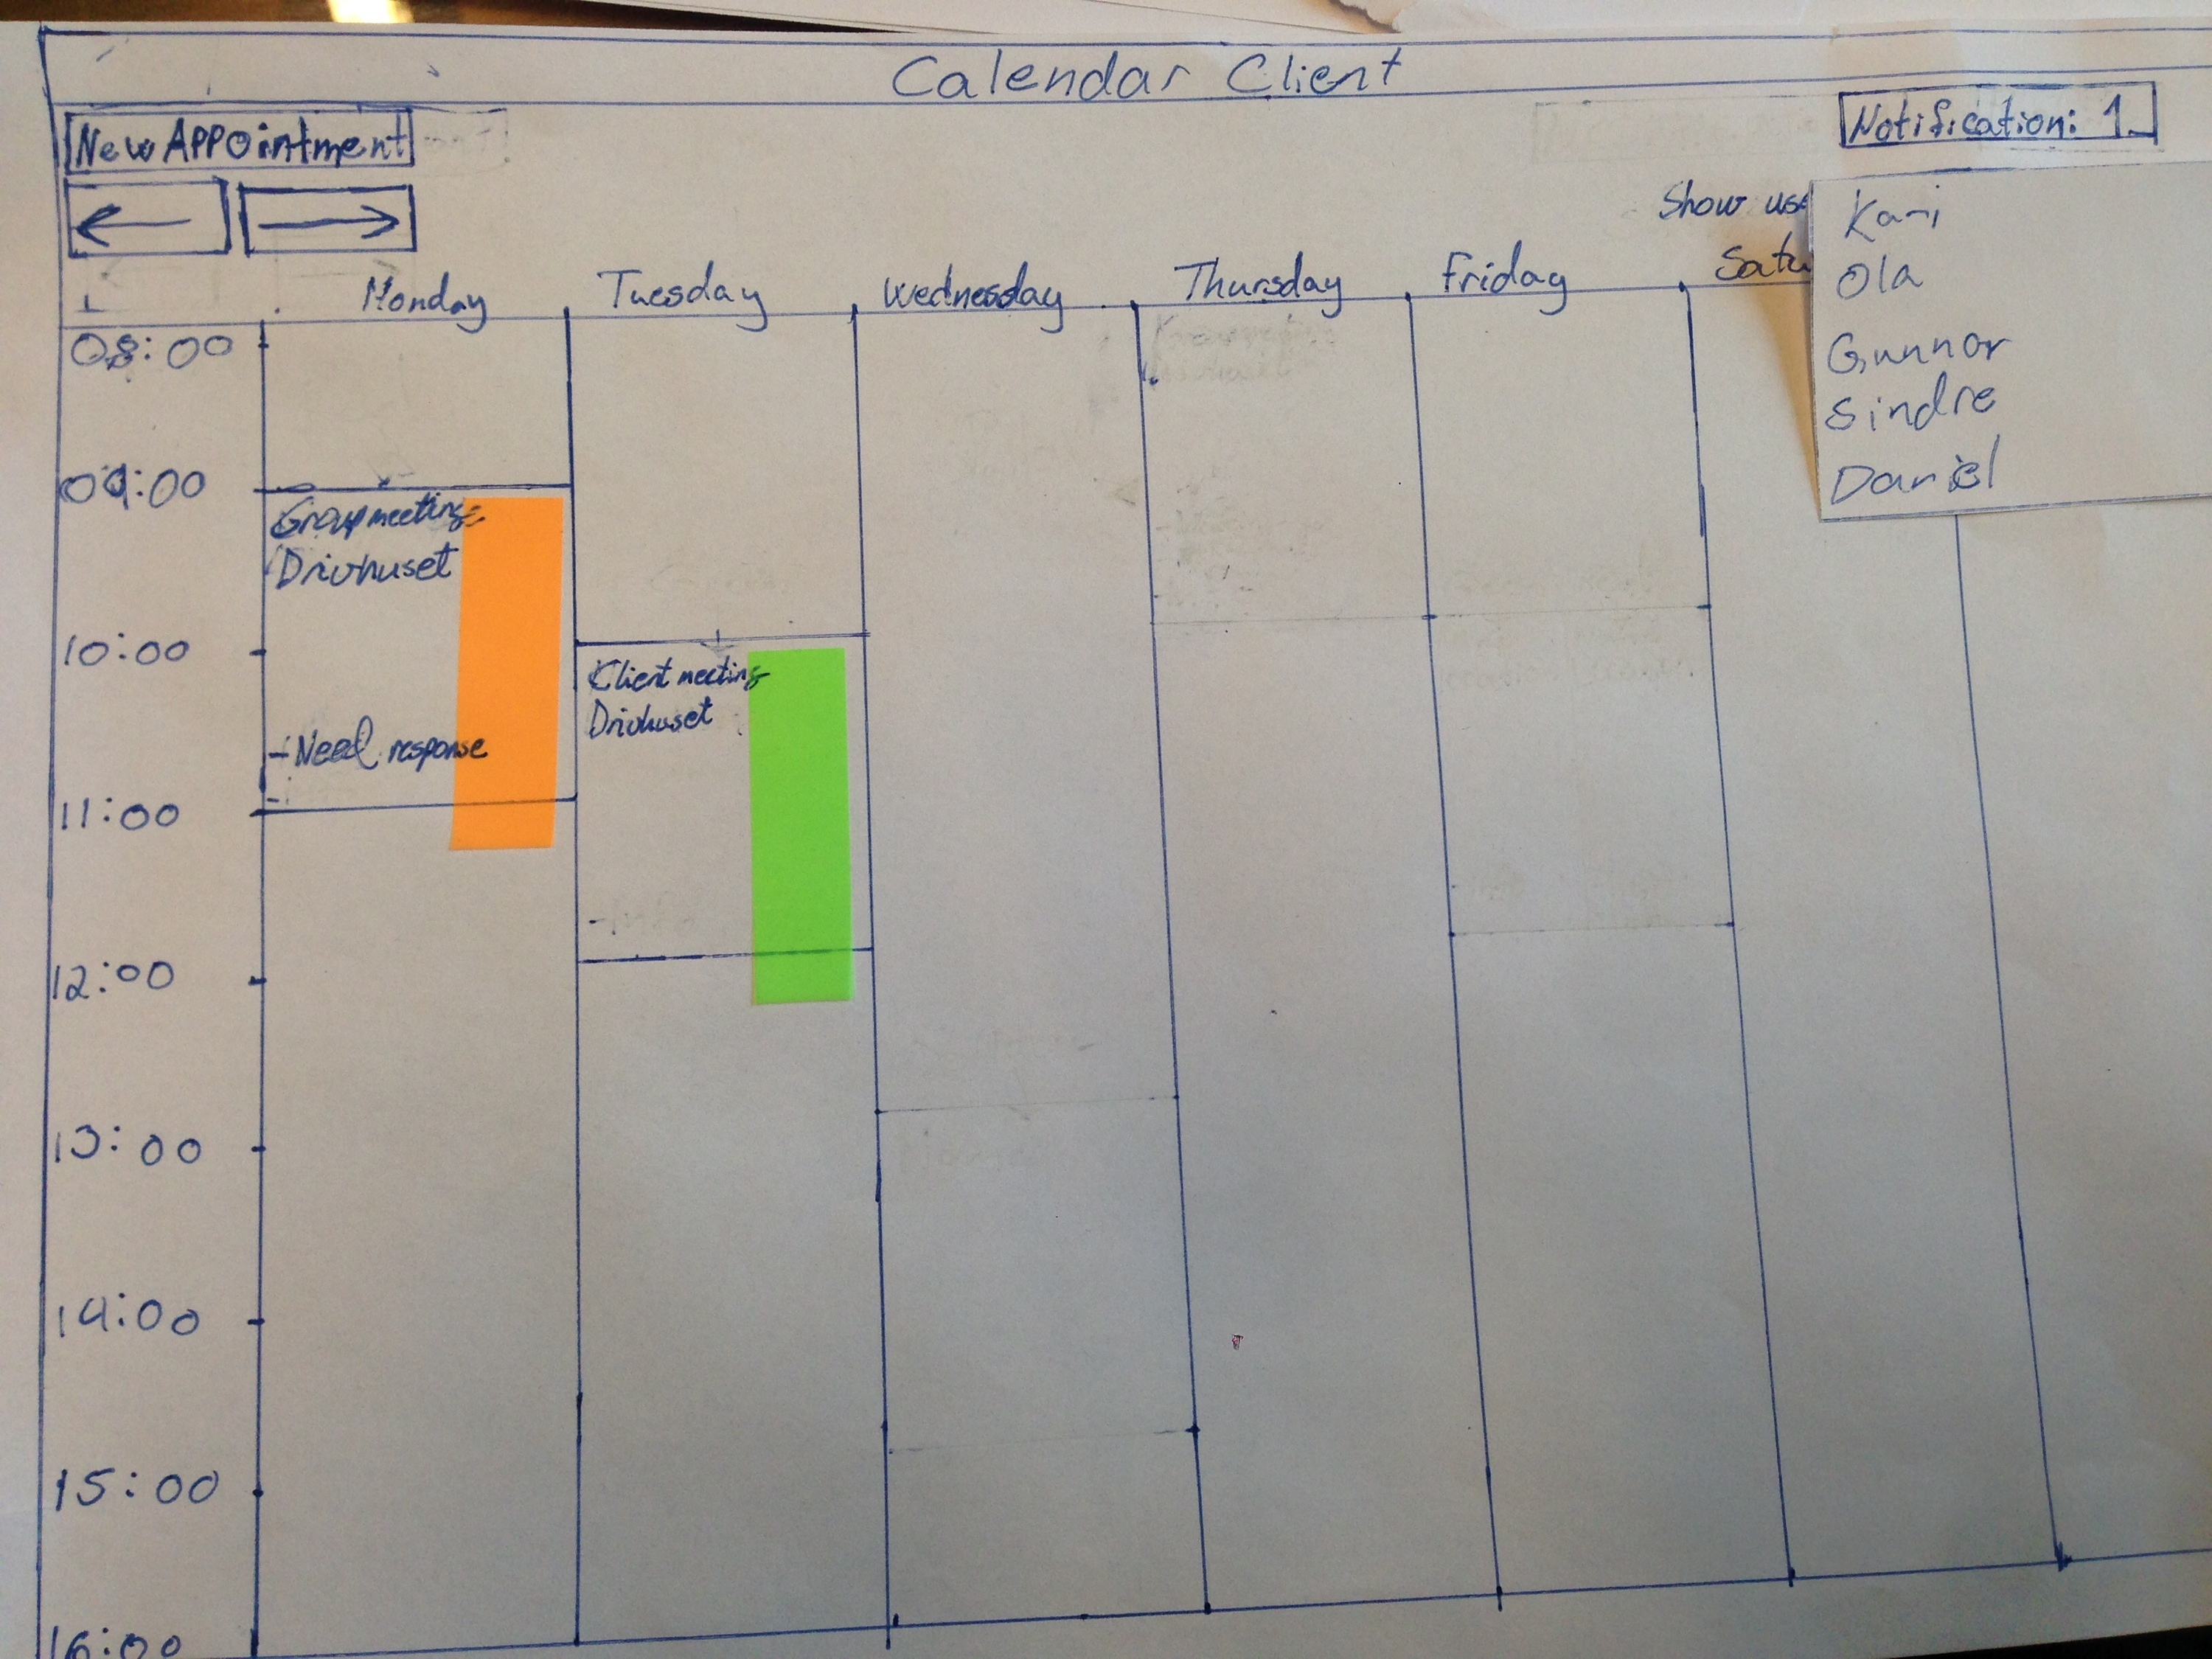
\includegraphics[width=8cm]{img/IMG_5610.JPG}
        \caption{Show user}
    \label{showuser}
    \end{center}
\end{figure}
``Show user'' is a JComboBox where the user can view other users calendar by selecting the name of the other user in the JComboBox.

\begin{figure}[h!] 
    \begin{center} 
        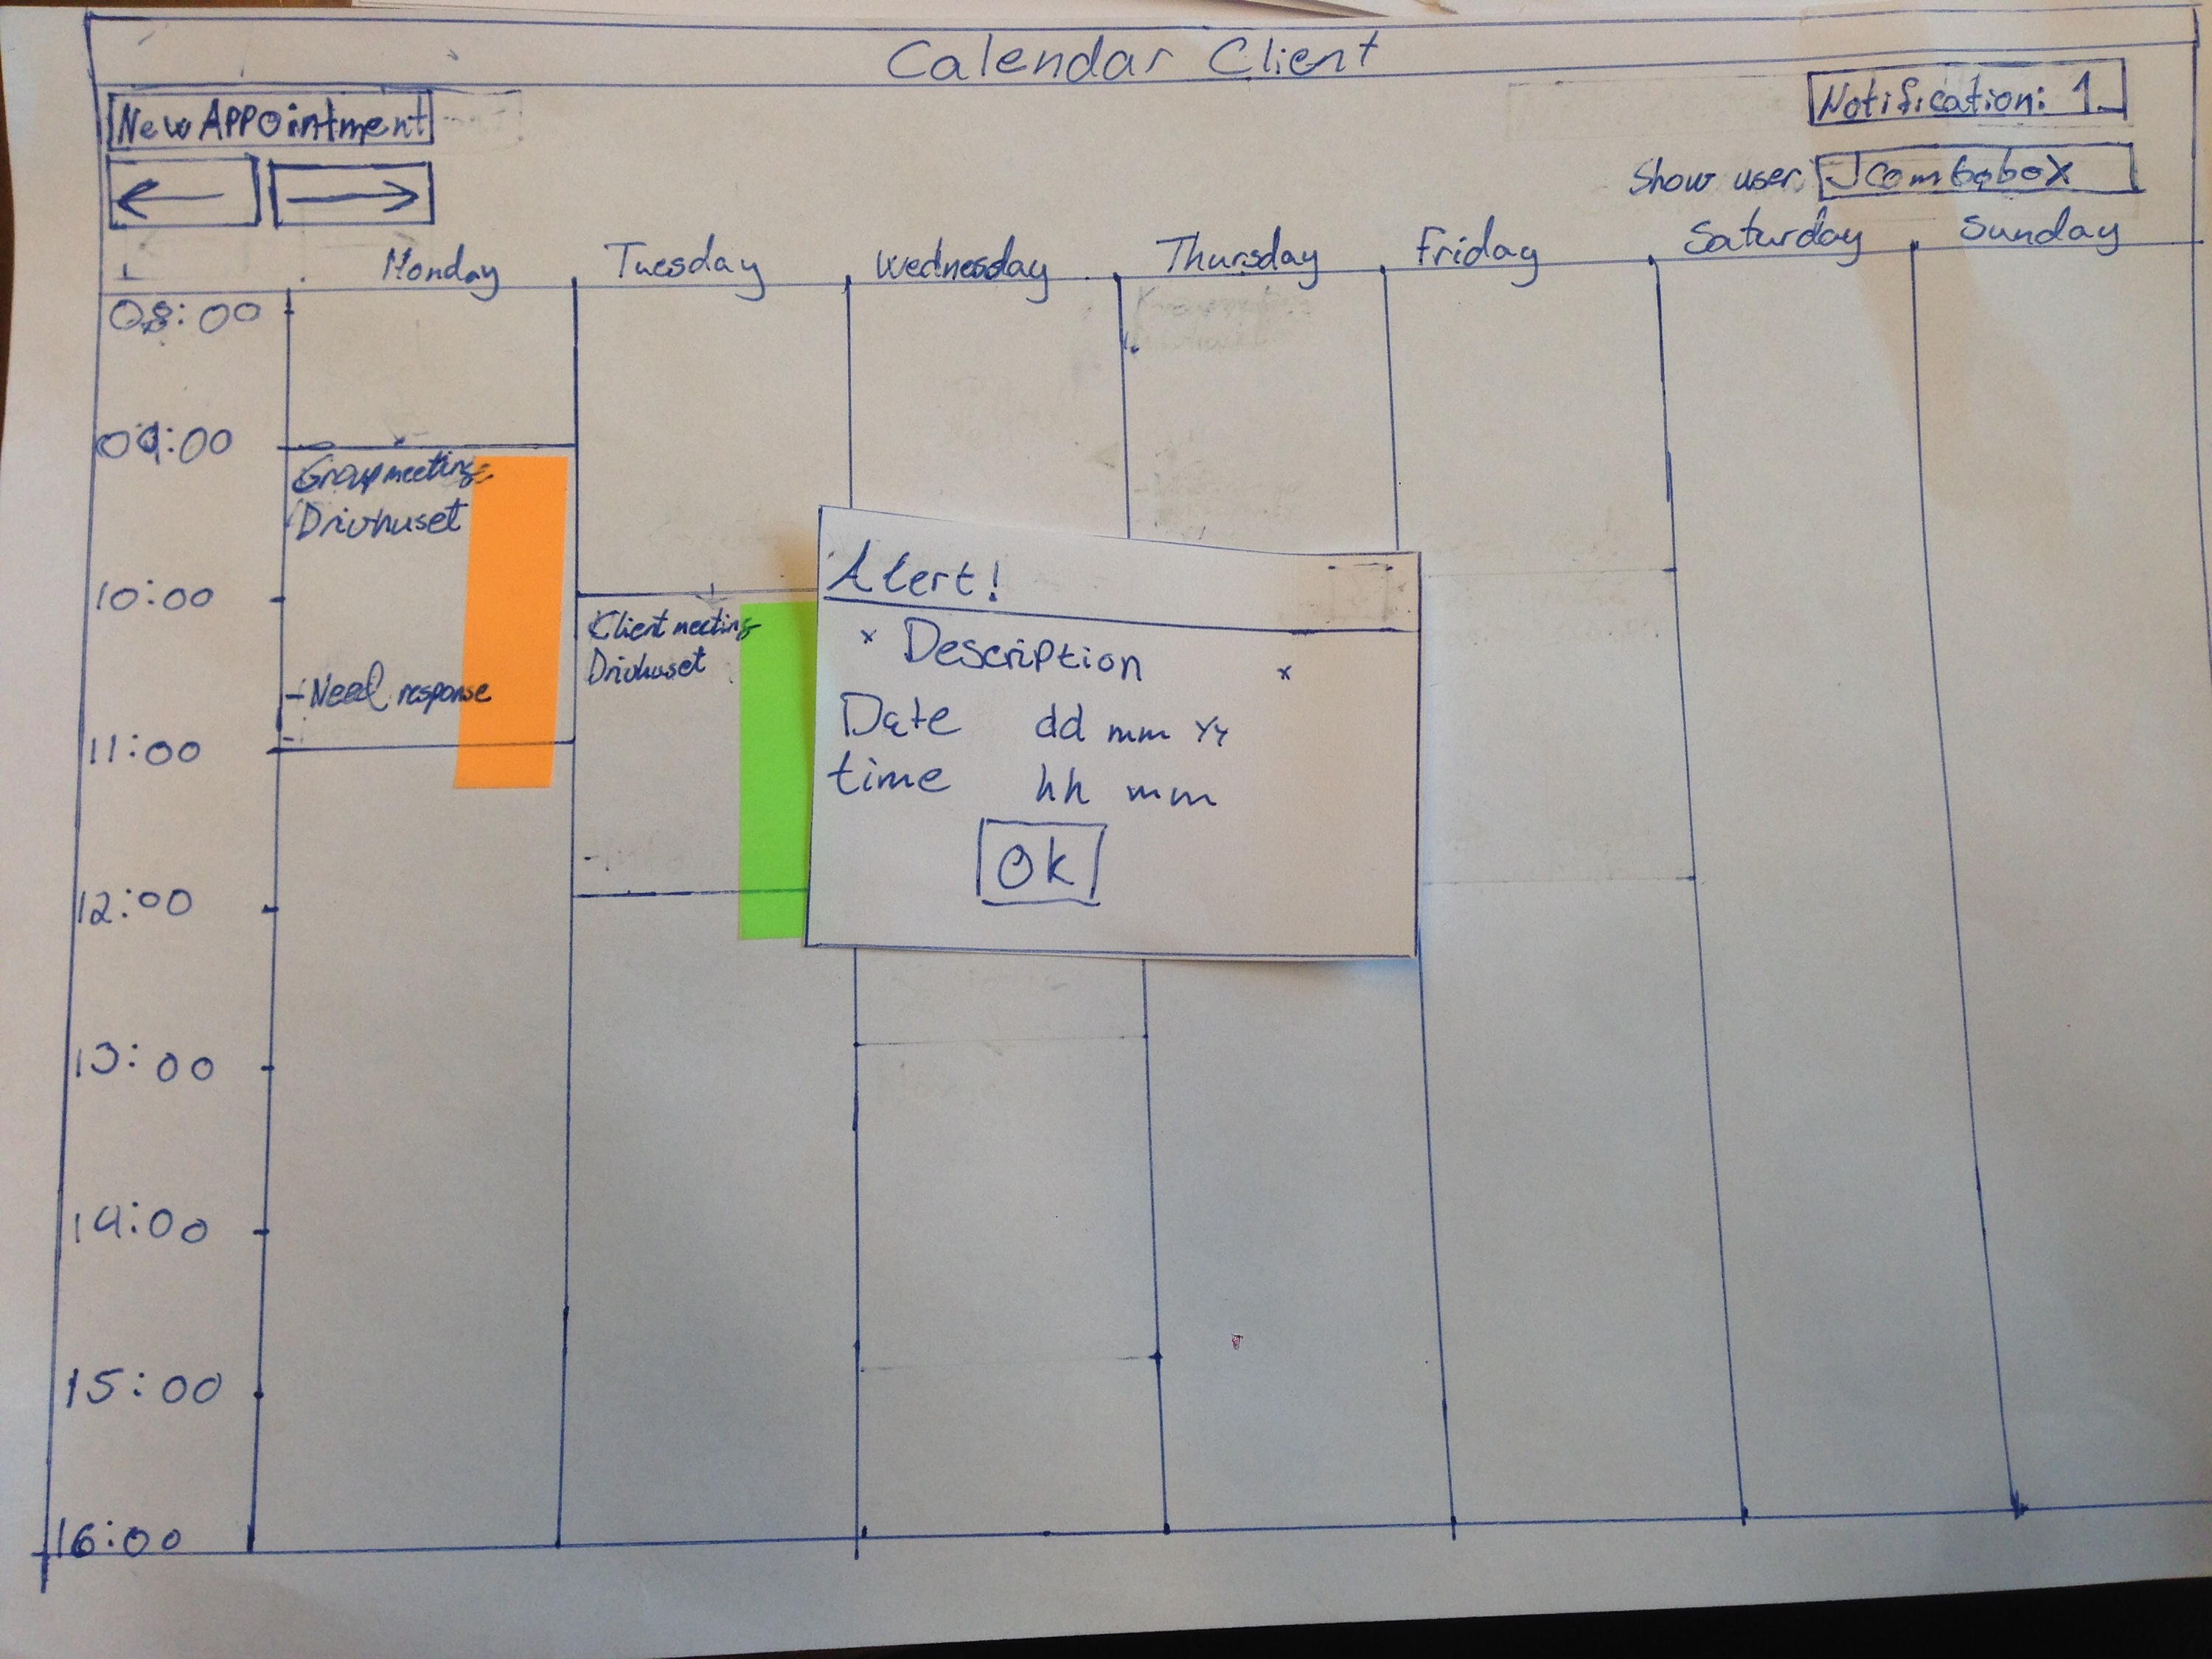
\includegraphics[width=8cm]{img/IMG_5611.JPG}
        \caption{Alarm popup}
    \label{alarm}
    \end{center}
\end{figure}
The alarm popup is a popup which appears when a alarm goes off. By pressing the ``OK''-button, the popup will close.

\newpage

\section{The task at hand}
A usability test was performed to test the paperprototype. The tasks was as follows:
\begin{enumerate}

\item You shall invite a business connection to a meeting in your companys own meetingrooms (already registered in the system). You will invite Kari to a meeting from 12:00 - 14:00, 10. march, and you're supposed to book a meeting room through this calendar system.

\item Kari has now received a phonecall. Unfortunately she have to go to another more imortant meeting at the time you invited her. You will now be Kari and decline the appointment you were invited to first.

\item You're yourself again, and you have received a notification. Check this.

\item Delete Kari from this meeting and and Sindre instead.

\item Yor businessconnection calls you, and tell you he's one hour late. Change this in the appointment in the calendar.
\end{enumerate}


Ole Halvor Dahl






\section{The test}
\subsection{With studentassistant}
\subsubsection*{Roles}
\begin{itemize}
\item Testleader: Jonas André Dalseth and Andreas Wien
\item Observers: Jonas André Dalseth, Finn Inderby, Espen Albert
\item Wizard Of Oz: Jonas André Dalseth og Andreas Wien
\item Tester: Fredrik Winther Dahl
\end{itemize}

\subsubsection*{Exectution}
The test with the student assistant wasn't very organized. First we thought we was just supposed to show him the paper model, so we didn't have any routines. Everybody on the group guided him through different scenarios, and we hadn't made any before we met him. After the test we asked him to fill out the SUS scheme and asked him what he thought about the system. We learned a lot about talking to him, and he told us how we should do it when we tested with the other group. 
\subsection{With other group}
\subsubsection*{Roles}
\begin{itemize}
\item Testleader: Jonas André Dalseth
\item Wizard of Oz: Andreas Wien
\item Observers: Finn Inderhaug, Kristoffer Dalby
\item Tester: Ole Halvor Dahl
\end{itemize}

\subsubsection*{Execution}
We met another group also working with the common project. The other group had chosen one person who would test our system. We chose one test leader, one "wizard of oz" and two people who wrote down the results from the test. The testleader presented how the test will work, what we are testing and how we are gonna do it. The test started, and the tester did the task presented above, without help from anyone of us. When the test was finished, he filled in a SUS diagram, and we asked him what he thought about the system.

\section{Results}
\subsection{With Student assistant}
Our student assistant gave us a lot of valued response on both how we executed the test and how our system worked. The changes suggested to our execution were extremely helpful before our second testgroup, and included the following:
\begin{enumerate}
\item Select a test leader and a person to serve as your system.
\item Test leader should introduce the test, pointing out that it's the system that's being tested. 
\item Test subject should be given a set of scenarios or tasks to properly test the system. 
\item Test subject should be informed that (s)he may abort the test at any time.
\item Test subject should not be assisted in any way once the test starts.
\item Only the test leader should hold a dialog with the test subject.
\item The remaining members should be observing and noting any difficulties occuring during the test.
\end{enumerate}

The suggestions for the paper prototype included the following points:
\begin{enumerate}
\item The notifications popup was a bit difficult to understand because of a lack of division between elements in the list.
\item There was no support for clicking at a desired time and date directly in the calendar to create a new appointment.
\item When editing or creating an appointment the list of meeting rooms didn't show how many participants a room could hold.
\item When editing or creating an appointment it's not intuitive how to add more members.
\end{enumerate}

\subsection{With other group}
\begin{enumerate}
\item The test subject could not find the dates for the weekdays in the calendar view.
\end{enumerate}

\section{Redesign}
\begin{enumerate}
\item Make it possible for one notification to take more space than one line, and make them more separated.
\item This is a extra feature, so we will only implement it if we get time to do it
\item Make a add all alternative in JComboBox
\item The view will be changed so the size of the room will appear in the JComboBox, such that it appears next to the name om the meeting room
\item Show dates next to the days in the calendar






\end{document}